This chapter covers what was actually built and run: the installed application, how the dataset was produced in practice, the two training runs, the exported model, and the things that went wrong along the way. The design reasoning behind these choices is in Chapter~III; the results they produced are in Chapter~V.

\section{The Installed Application}

The application installs as \texttt{vnphish} and has three commands. The one that matters is:

\begin{quote}
\texttt{vnphish analyze --text "<message>"}
\end{quote}

\noindent This takes one Vietnamese message and prints the result. The other two are support commands: \texttt{vnphish doctor} checks that the model and settings loaded correctly before anything is analysed, and \texttt{vnphish demo} opens the same analysis in a local browser page for demonstration.

The source tree is organised by what each part does:

\begin{quote}
\begin{verbatim}
src/
  core/             strict JSON validation and safe file writes
  artifacts/        reading model and result files
  config/           local settings
  data_pipeline/    building the dataset: records, text handling,
                    splitting, generation, judging, one-off repairs
  modeling/         training, inference and evaluation
  runtime/          the CLI, the analysis service, the demo page
  source_archiving/ keeping a fixed copy of the source
  model_adaptation/ the older experiment code, kept for reference
\end{verbatim}
\end{quote}

\noindent New work goes through \texttt{modeling}. The older \texttt{model\_adaptation} code is kept because the completed experiments were run with it, and it is what the recorded results actually came from. Keeping the two apart avoids implying that later tidying produced earlier numbers.

\section{Building the Dataset}

Every message carries the \texttt{seed\_id} of the article it was written from, and the splitter sends all messages sharing an ID into one split. That rule is stricter than splitting message by message, and it is what stops a reworded message from appearing on both sides of the evaluation.

The first pass was generated by Claude 3.5 Haiku, one class at a time. Reviewing it showed that a large part was not usable. One whole group of Zalo messages had been written as third-person narration, describing a scam rather than being one. Other classes carried leftover template text: bracketed placeholders such as \texttt{[CCCDUpdateApp]}, unresolved URLs such as \texttt{[http://xyz-bank-update.com]}, and obviously fake domains such as \texttt{fake-bank.vn}.

Those messages were rewritten rather than patched. The replacements were produced offline from a fixed local catalogue built from the original article scenarios, so no external API call was made during the repair. They then went through the same automatic checks as everything else.

A judge model scored every message, and a Vietnamese-speaking reviewer checked a sample by hand and worked through the messages whose labels looked wrong. What the checks found is reported in Chapter~V.

\section{Measuring LoRA Against QLoRA}

Both training methods were run briefly on the target laptop before either was committed to. These were short measurement runs, not attempts to train a usable model, and the adapters they produced were deleted afterwards.

\subsection{Ordinary LoRA}

The LoRA run recorded 31 optimizer steps, 26 of them measured. It ran for 1{,}782.206~seconds, just under thirty minutes, with a median step of 53.274~seconds. Multiplying that median across the planned 1{,}245-step schedule gives roughly 18.42~hours of computation, and the mean-step version gives 18.88~hours. Neither figure includes the time spent on validation and saving checkpoints, so neither is a prediction of how long the run would actually take.

Memory was the deciding factor. The card holds 8{,}151~MiB, and at its tightest moment \texttt{nvidia-smi} reported only 9~MiB of it still free.

The run did real optimizer work with sensible losses and did \emph{not} produce an out-of-memory error, and this report does not claim it did. It stopped early for an unrelated controller fault. The problem is the combination: an eighteen-hour run with almost no memory to spare is a bad bet, because any brief extra allocation would end it and cost most of a day.

\subsection{NF4 QLoRA}

The QLoRA run confirmed that 4-bit NF4 was genuinely active: 252 four-bit layers, a frozen base model, and 504 trainable adapter tensors. It completed five warm-up steps plus 40 measured ones, with a median step of 3.462389~seconds.

Memory peaked at 7{,}516 of 8{,}151~MiB, leaving a workable margin throughout, and no out-of-memory error or thermal stop occurred. Figure~\ref{fig:resource-probe-comparison} compares the two runs, and Figure~\ref{fig:probe-console} is the console output as it appeared while this one was running.

\begin{figure}[H]
\centering
\begin{tikzpicture}[
  metric/.style={font=\small\bfseries, anchor=east},
  value/.style={font=\scriptsize, anchor=west},
  legend/.style={font=\small, anchor=west}
]
\fill[CVBLUE!80] (0,6.55) rectangle (0.35,6.82);
\node[legend] at (0.48,6.685) {ordinary LoRA probe};
\fill[orange!80] (4.0,6.55) rectangle (4.35,6.82);
\node[legend] at (4.48,6.685) {NF4 QLoRA probe};

\node[metric] at (-0.20,5.45) {Median step};
\fill[CVBLUE!80] (0,5.55) rectangle (4.79,5.83);
\fill[orange!80] (0,5.12) rectangle (0.31,5.40);
\node[value] at (4.90,5.69) {53.274 s};
\node[value] at (0.42,5.26) {3.462 s};

\node[metric] at (-0.20,3.95) {Projected schedule};
\fill[CVBLUE!80] (0,4.05) rectangle (5.53,4.33);
\fill[orange!80] (0,3.62) rectangle (0.36,3.90);
\node[value] at (5.64,4.19) {18.42 h};
\node[value] at (0.47,3.76) {1.21 h};

\node[metric] at (-0.20,2.45) {Peak VRAM};
\fill[CVBLUE!80] (0,2.55) rectangle (5.82,2.83);
\fill[orange!80] (0,2.12) rectangle (5.53,2.40);
\node[value] at (5.93,2.69) {7,902 / 8,151 MiB};
\node[value] at (5.64,2.26) {7,516 / 8,151 MiB};

\node[metric] at (-0.20,0.95) {Minimum free VRAM};
\fill[CVBLUE!80] (0,1.05) rectangle (0.14,1.33);
\fill[orange!80] (0,0.62) rectangle (5.93,0.90);
\node[value] at (0.25,1.19) {9 MiB};
\node[value] at (6.04,0.76) {395 MiB};

\draw[black!35] (0,0.40) -- (0,6.10);
\end{tikzpicture}
\caption{Bounded RTX 5050 resource probes. Step time and optimizer-schedule duration use separate visual scales; the duration values are projections, not observed end-to-end runtimes. Neither probe produced an out-of-memory event.}
\label{fig:resource-probe-comparison}
\end{figure}


\begin{figure}[H]
\centering
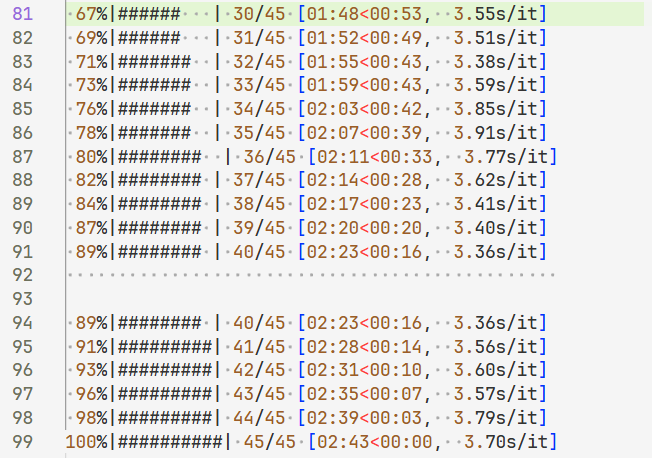
\includegraphics[width=0.80\linewidth]{figures/training_console_probe.png}
\caption{Console output from the 45-step QLoRA measurement run. The bar reaches 45 of 45 steps at 2~minutes 43~seconds, and the 3.70~s/it it reports is its own running average across all 45, including the five warm-up steps; the 3.462389~s quoted above is the median of the 40 steps after warm-up. The run's total was 3~minutes 42~seconds, and the extra 59~seconds is the closing validation pass and checkpoint save. This is the short measurement run, not the full training run.}
\label{fig:probe-console}
\end{figure}

\section{Training Qwen}

The full Qwen run used the 1{,}658 training and 219 validation messages, three epochs, and 1{,}245 optimizer steps from a fresh start. The package versions were Python~3.13.13, PyTorch~2.12.0+cu132, Transformers~5.9.0, PEFT~0.19.1, and bitsandbytes~0.50.1.

The model was evaluated every 50 steps, and the checkpoint that scored best on the validation messages was kept. That turned out to be step 200. Later checkpoints trained longer but did not score better, which is what the evaluation sweep in Figure~\ref{fig:checkpoint-sweep} shows. The loss curves for the run are in Figure~\ref{fig:qwen-training-curves}.

\begin{figure}[H]
\centering
{\small\bfseries Qwen QLoRA training curves\par}
\smallskip
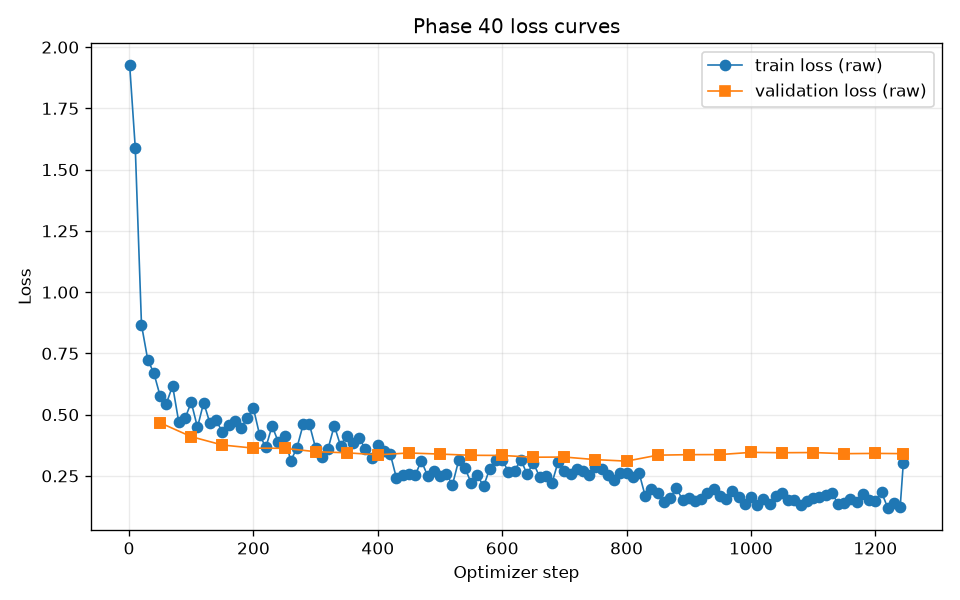
\includegraphics[width=0.91\linewidth,trim=0 0 0 24bp,clip]{figures/qwen_loss_curves.png}
\caption{Qwen QLoRA training and validation loss across the completed 1{,}245-step run.}
\label{fig:qwen-training-curves}
\end{figure}

The run took 14.87 hours from start to finish, but most of that was not training. The 1{,}245 optimizer steps account for only 1.36 hours. The rest is validation: at each of the 25 checkpoints the model had to write a full structured answer for all 219 validation messages, which is 5{,}475 generated answers on a laptop GPU. Figure~\ref{fig:run-timeline} shows this as a staircase, where each flat section is one validation pass.

\begin{figure}[H]
\centering
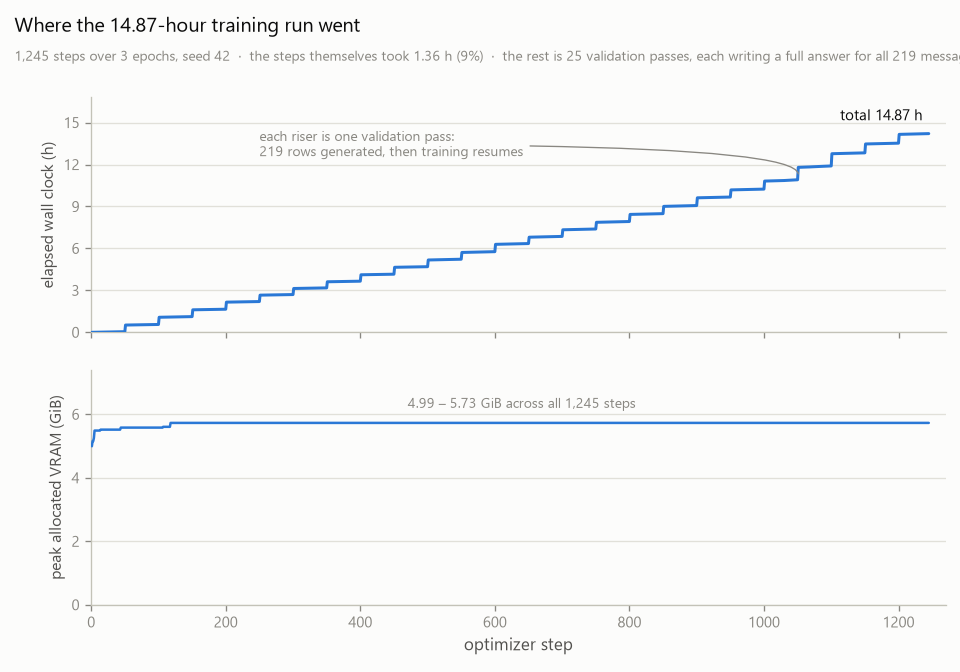
\includegraphics[width=0.92\linewidth]{figures/full_run_timeline.png}
\caption{Where the 14.87 hours went, and how much memory PyTorch itself held during the run. The lower panel reports PyTorch's own allocation, which is smaller than the whole-card figure of 7{,}516~MiB quoted for the measurement runs above: that figure came from \texttt{nvidia-smi} and includes memory held by the driver and the display as well as by training.}
\label{fig:run-timeline}
\end{figure}

\section{Training PhoBERT}

PhoBERT was trained separately on the same messages as a full four-class classifier, with nothing quantized and no adapter. The run took 312 steps, and the checkpoint at step 100 was kept. Its loss curves are in Figure~\ref{fig:phobert-training-curves}.

The result is an ordinary Transformers bundle: a 540~MB \texttt{model.safetensors} weights file with its tokenizer and configuration files, and a 1.03~GB optimizer state saved alongside it. PhoBERT was not converted to GGUF.

\begin{figure}[H]
\centering
{\small\bfseries PhoBERT training curves\par}
\smallskip
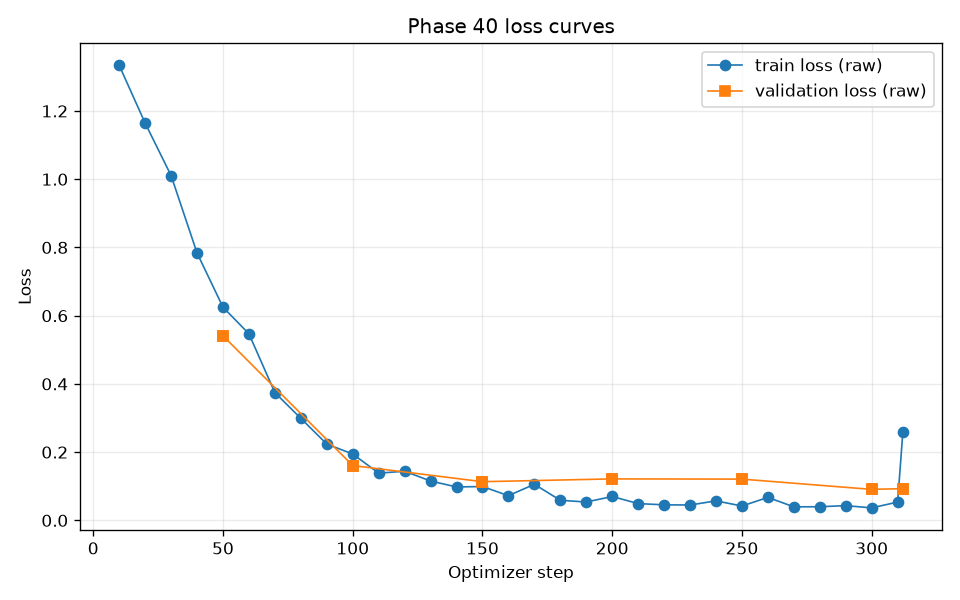
\includegraphics[width=0.91\linewidth,trim=0 0 0 24bp,clip]{figures/phobert_loss_curves.png}
\caption{PhoBERT training and validation loss across the completed 312-step run.}
\label{fig:phobert-training-curves}
\end{figure}

\begin{figure}[H]
\centering
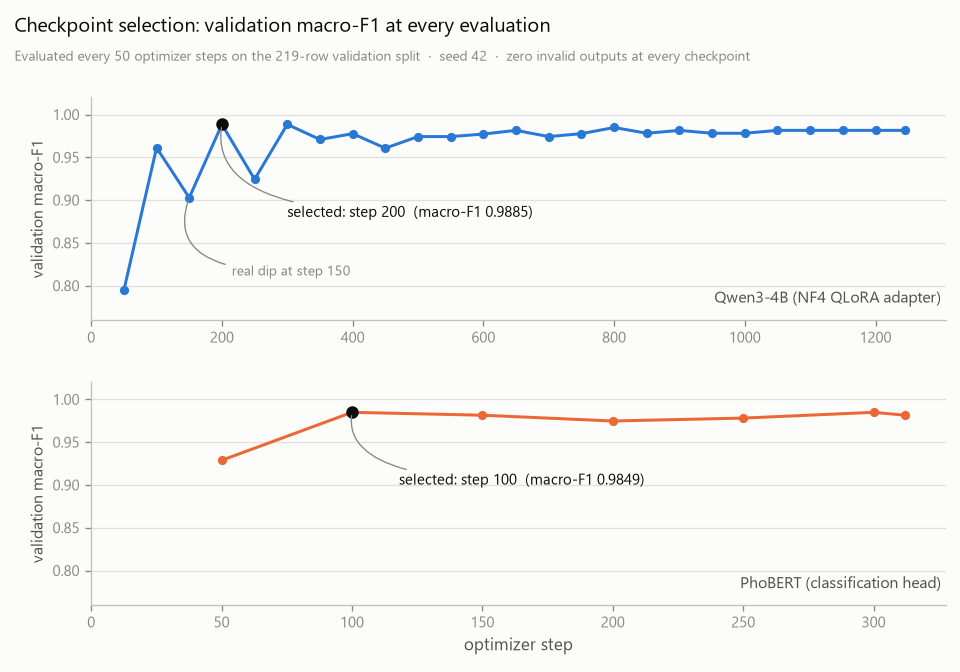
\includegraphics[width=0.92\linewidth]{figures/checkpoint_selection_sweep.png}
\caption{Validation score at every checkpoint of both runs, with the selected checkpoint marked. Qwen was evaluated 25 times across its 1{,}245 steps and PhoBERT 7 times across its 312.}
\label{fig:checkpoint-sweep}
\end{figure}

\section{Exporting the Model}

The trained Qwen adapter was merged back into its base model and converted through \texttt{llama.cpp} \cite{gerganov2023llamacpp} into one Q8\_0 GGUF file of 4{,}280{,}403{,}232 bytes. It was then loaded twice, once independently, to confirm the exported file works.

Figure~\ref{fig:artifacts-on-disk} shows everything the two runs left on disk, the export included.

At runtime the analysis service normalises the message text, sends it to whichever model is configured, and returns the risk tier, threat label, quoted evidence, and recommendations. Nothing in this path needs an API key or an internet connection.

\begin{figure}[H]
\centering
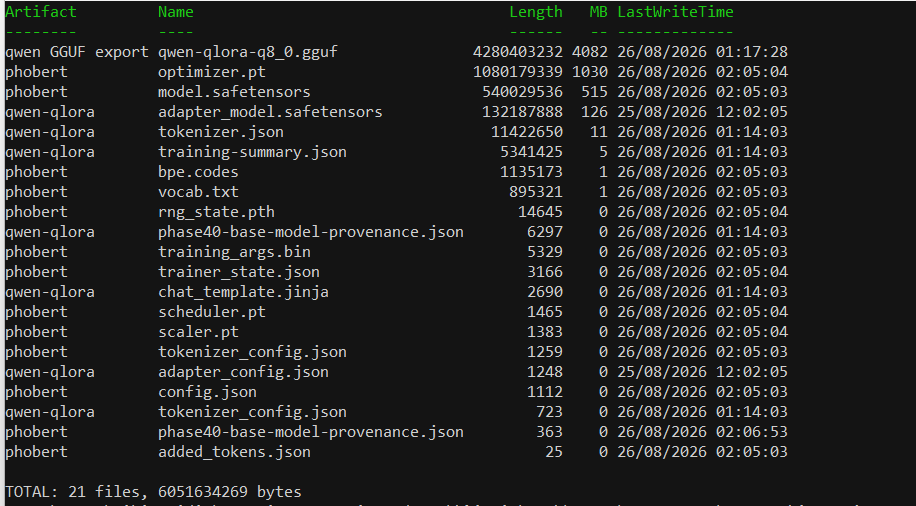
\includegraphics[width=0.95\linewidth]{figures/model_files_on_disk.png}
\caption{Everything the two training runs left on disk, with the exported model: 21 files, 6{,}051{,}634{,}269 bytes in total. The GGUF export alone accounts for 4{,}280{,}403{,}232 of them.}
\label{fig:artifacts-on-disk}
\end{figure}

\section{What Went Wrong, and What Was Done About It}

Three failures shaped this project more than any of the successes, so all three are recorded here.

\textbf{Generation kept dying part-way through.} The first dataset pass ran for a long time against an external API, and interruptions lost everything generated up to that point. The fix was to write checkpoint files as generation proceeded, so a failure costs the last few minutes rather than the whole run.

\textbf{A large part of the generated data was unusable.} As described above, one class had been written as narration and others carried template leftovers. These were found by reviewing the output rather than by any automatic check, which is the argument for reading generated data rather than trusting it.

\textbf{Ordinary LoRA was not practical on this hardware.} The measurement run left almost no spare memory and pointed at an eighteen-hour schedule. Rather than start it and hope, the project switched to QLoRA, which finished in a fraction of the time with room to spare.

Figure~\ref{fig:failure-recovery-timeline} puts all of them in the order they happened.

One more failure has to be named, because it affected the results directly. An early attempt at the full Qwen run was stopped deliberately after two defects appeared in how output folders and validation files were named. Nothing from that attempt was carried into the final run, which restarted from the beginning.

\begin{figure}[H]
\centering
\begin{tikzpicture}[
  event/.style={draw=orange!70!black, fill=orange!8, rounded corners=3pt,
    text width=2.55cm, minimum height=1.45cm, align=center, font=\scriptsize,
    inner sep=4pt},
  fix/.style={draw=green!55!black, fill=green!7, rounded corners=3pt,
    text width=2.55cm, minimum height=1.45cm, align=center, font=\scriptsize,
    inner sep=4pt},
  arr/.style={-{Stealth[length=2.4mm,width=1.8mm]}, line width=0.8pt, black!45,
    shorten >=1pt, shorten <=1pt},
]

%% row 1 --- building the dataset
\node[event] (a1) at (-5.55, 0)     {Generation run against an external API};
\node[event] (a2) at (-1.85, 0)     {Provider stopped accepting requests};
\node[event] (a3) at ( 1.85, 0)     {Results written only at the end, so the run was lost};
\node[fix]   (a4) at ( 5.55, 0)     {Retry with backoff, and results saved as they are produced};

%% row 2 --- repairing the dataset, then choosing the training method
\node[event] (b1) at (-5.55, -2.20) {One group of Zalo messages written as narration};
\node[fix]   (b2) at (-1.85, -2.20) {Rewritten offline from the stored scenarios};
\node[event] (b3) at ( 1.85, -2.20) {Ordinary LoRA left 9~MiB free and pointed at 18 hours};
\node[fix]   (b4) at ( 5.55, -2.20) {QLoRA fits the card with room to spare};

%% row 3 --- the training run itself
\node[event] (c1) at (-5.55, -4.40) {Output folder name left out the run ID};
\node[fix]   (c2) at (-1.85, -4.40) {Stopped on purpose and restarted from step zero};
\node[fix]   (c3) at ( 1.85, -4.40) {Both models trained to completion};

\draw[arr] (a1)--(a2);  \draw[arr] (a2)--(a3);  \draw[arr] (a3)--(a4);
\draw[arr] (a4.south) -- ++(0,-0.55) -| (b1.north);
\draw[arr] (b1)--(b2);  \draw[arr] (b2)--(b3);  \draw[arr] (b3)--(b4);
\draw[arr] (b4.south) -- ++(0,-0.55) -| (c1.north);
\draw[arr] (c1)--(c2);  \draw[arr] (c2)--(c3);

\end{tikzpicture}
\caption{The order in which things went wrong, and what was changed after each one. Orange is a failure, green is the fix that followed it. Each row is one stage of the work: building the dataset, repairing it and choosing a training method, and the training run itself.}
\label{fig:failure-recovery-timeline}
\end{figure}

